\chapter{What Communication Requires}

This chapter follows J. Krishnamurti's 1974 San Diego dialogue with Allan W. Anderson on communication, relationship, seriousness, responsibility, and negation. The source is a spoken inquiry rather than a blackboard lecture, so the displayed formulas below are not imported mathematics. They are compact maps of the dialogue's logical movement, useful only when they keep the distinctions clear. Credit belongs to J. Krishnamurti and the Krishnamurti Foundation Trust source material, with curation by LazyingArt LLC through Video2Book.

\section{The Right Beginning}

Anderson opens by recalling a discipline from the previous conversation: one must not finish by theoretical construction before finding the right beginning. That caution sets the method for the whole chapter. We are not trying to build a system around communication. We are trying to begin where communication actually begins.

The proposed topic is communication, but Krishnamurti immediately adds relationship. Communication is not an isolated event between two separate minds. It takes place, if it takes place at all, in relationship. The first move, then, is to refuse the usual picture in which one person makes a statement and the other accepts, rejects, compares, or stores it.

A compact way to record the first distinction is
\begin{equation}
\text{communication}
\approx
\text{verbal understanding}
+
\text{non-verbal communion}.
\end{equation}
This equation is only a notation for the inquiry. Words matter, but words by themselves do not constitute communication.

\begin{definition}
In this chapter, \emph{communication} means the shared movement of speaking, listening, observing, and thinking together. It is not mere information transfer, and it is not the delayed reaction of agreement or disagreement.
\end{definition}

The definition is dynamic. Communication is not a result reached after a successful discussion. It is the condition under which the inquiry can begin.

\section{Listening As Shared Attention}

Once communication is joined to relationship, the word opens into the art of listening. Krishnamurti is not asking for a technique of interpretation. He is asking whether there can be listening without the immediate movements of acceptance, denial, comparison, and judgment.

The lecture gives us a useful simultaneity condition:
\begin{equation}
\text{same level}
+
\text{same time}
+
\text{same intensity}
\Longrightarrow
\text{walking together}.
\end{equation}
The image of walking together is exact. It prevents the false model in which one person speaks, the other thinks about it later, and communication is postponed until a judgment has formed. Krishnamurti is describing concurrent activity.

The inner movement can be written as
\begin{equation}
\text{listening}
\xrightarrow{\ \text{attention}\ }
\text{insight}.
\end{equation}
The essential point is that insight is not set aside as a reward at the end. Anderson notices this: the insight must be present from the beginning as the two inquire together.

\begin{figure}
\centering
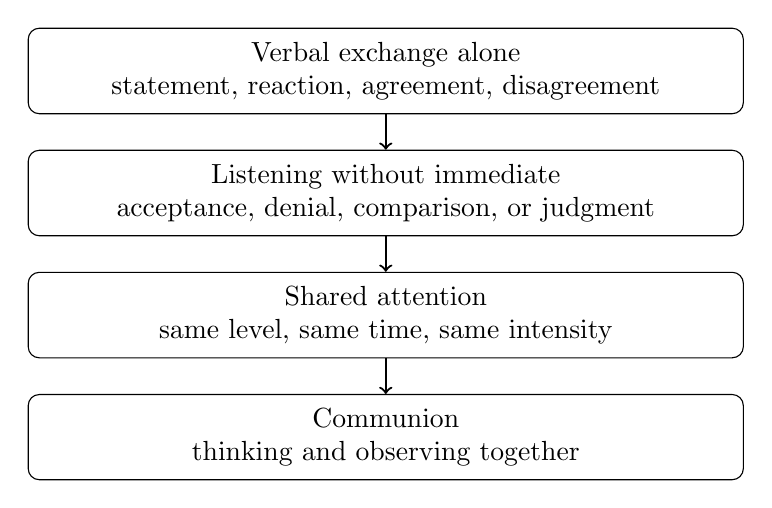
\begin{tikzpicture}[
  every node/.style={draw, rounded corners, align=center, text width=0.72\linewidth, inner sep=5pt},
  arrow/.style={->, thick}
]
\node (a) at (0,0) {Verbal exchange alone\\statement, reaction, agreement, disagreement};
\node (b) at (0,-1.55) {Listening without immediate\\acceptance, denial, comparison, or judgment};
\node (c) at (0,-3.10) {Shared attention\\same level, same time, same intensity};
\node (d) at (0,-4.65) {Communion\\thinking and observing together};
\draw[arrow] (a) -- (b);
\draw[arrow] (b) -- (c);
\draw[arrow] (c) -- (d);
\end{tikzpicture}
\end{figure}

The diagram is an editorial map, not a reconstruction of a board. It keeps the lecture's first progression visible: from words, to listening, to attention, to communion.

The pivot to communion is important. Anderson suggests that communication and communion are deeply related. Krishnamurti accepts this, but only under a condition: both must be serious about the same problem, with the same passion. If one is not interested, communication stops. If one is merely entertained, communication stops. Communion requires seriousness.

\section{Seriousness Without Grimness}

The next obstacle lies in the word ``serious.'' Anderson observes that ordinary usage often makes seriousness sound like pain, heaviness, or effort for the sake of getting something. Krishnamurti refuses that meaning. To be serious is not to be long-faced, miserable, or ambitious for a result. It means that the problem is real and cannot be played with.

The example is medical and immediate. If one has cancer, one does not treat it as entertainment. The seriousness belongs to the fact that it must be understood and acted upon.

\subsection{Question \& Answer}

\paragraph{Question.}
Does seriousness mean effort stretched out over time?

\paragraph{Answer.}
No. In the dialogue, seriousness is not the promise that one will act later. It is the quality of seeing the problem as actual. When the seeing is serious, action is not deferred.

The contrast is sharp:
\begin{equation}
\text{doing} \neq \text{``I will do''}.
\end{equation}
The phrase ``I will do'' already opens psychological time. It has moved away from the fact and into postponement. Krishnamurti's stronger claim is
\begin{equation}
\text{clear seeing}
\Longrightarrow
\text{immediate action}.
\end{equation}

\begin{proposition}
In this lecture, seriousness is not a mood. It is the inseparability of seeing and action before a real crisis.
\end{proposition}

\begin{proof}
The dialogue first distinguishes seriousness from pain, grimness, and wanting something from the situation. It then places seriousness in relation to a world of disorder for which the human being is responsible. A serious problem is not deferred. Therefore the action appropriate to seriousness is immediate, not the delayed action of an ideal future.
\end{proof}

Krishnamurti then gathers the elements of seriousness: intent, urge, total responsibility, action, and doing. The phrase ``not, I will do'' is the hinge. Seriousness is not the projection of action into time; it is the demand of the fact.

\section{Responsibility As Adequate Response}

Anderson next selects one term inside seriousness: responsibility. He hears the word as the ability to be responsive. Krishnamurti accepts the direction and gives it precision. Responsibility means responding adequately to a challenge.

The challenge is not abstract. The world is confused, sorrowful, violent, and disorderly. The human being has helped create this disorder. To be responsible is not to feel vague guilt, and it is not to devise a plan from outside the problem. It is to respond to the problem itself.

We can write the working definition as
\begin{equation}
\text{responsibility}
=
\text{adequate response to challenge}.
\end{equation}

Now the difficulty appears. We rarely respond to the challenge. We respond to our conclusion about the challenge. A plan is superimposed; if the plan fails, we blame ourselves or change the plan. But the plan has already displaced the fact.

The structure of displacement is
\begin{equation}
\text{challenge}
\xrightarrow{\ \text{conclusion, plan, fear, pleasure, past}\ }
\text{translated response}
\neq
\text{adequate response}.
\end{equation}

\begin{figure}
\centering
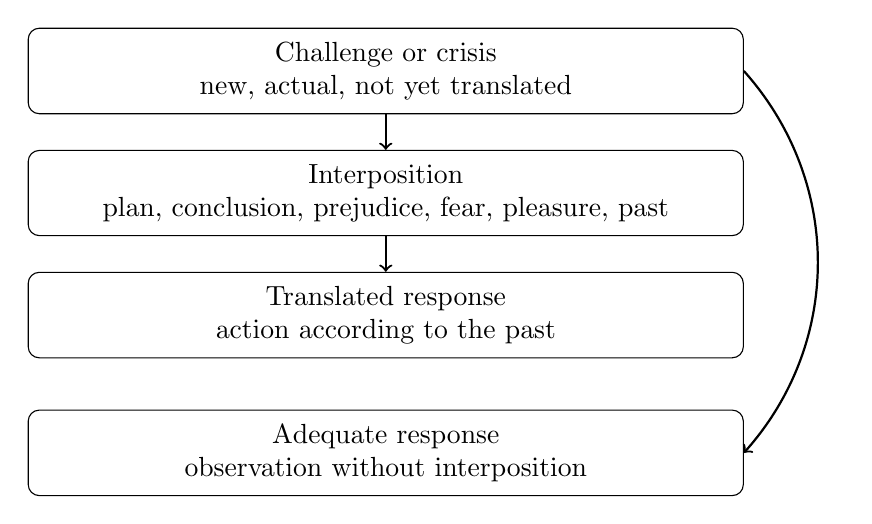
\begin{tikzpicture}[
  every node/.style={draw, rounded corners, align=center, text width=0.72\linewidth, inner sep=5pt},
  arrow/.style={->, thick}
]
\node (challenge) at (0,0) {Challenge or crisis\\new, actual, not yet translated};
\node (screen) at (0,-1.55) {Interposition\\plan, conclusion, prejudice, fear, pleasure, past};
\node (response) at (0,-3.10) {Translated response\\action according to the past};
\node (adequate) at (0,-4.85) {Adequate response\\observation without interposition};
\draw[arrow] (challenge) -- (screen);
\draw[arrow] (screen) -- (response);
\draw[arrow] (challenge.east) .. controls +(1.25,-1.4) and +(1.25,1.4) .. (adequate.east);
\end{tikzpicture}
\end{figure}

This is the lecture's first major structural problem. A response filtered through conclusion, inclination, fear, pleasure, belief, or memory is already a translation. It may be clever, sincere, or socially approved, but it is not adequate response.

\section{The Observer Is The Observed}

The statement ``the observer is the observed'' can sound like a doctrine if it is detached from its place in the lecture. Here it is earned by the failure of the separative model. The human being looks at the disorder of society and says, ``I must do something about it.'' Krishnamurti's reply is: the ``it'' is not separate from the human being who has created it.

In compact notation:
\begin{equation}
\text{observer} = \text{observed}.
\end{equation}
This is not a mathematical identity in the usual sense. It is an inquiry-formula: the one who observes the problem is not standing outside the problem.

The related formulation is
\begin{equation}
\text{world} = \text{me},
\qquad
\text{me} = \text{world}.
\end{equation}
Krishnamurti insists that this is not an intellectual or emotional conclusion. Within the dialogue it functions as a fact to be seen. Human beings, irrespective of labels, share the problems of relationship, suffering, jealousy, envy, greed, ambition, imitation, and conformity.

\subsection{Question \& Answer}

\paragraph{Question.}
If disorder continues far away, how can one say that the world is me and I am the world?

\paragraph{Answer.}
The objection already separates the person from the issue. Krishnamurti's answer is not that one private individual mechanically stops every outward event. Rather, he points to the common structure of human consciousness: fear, ambition, suffering, imitation, violence, and conformity are not private exceptions. They are shared human facts. To see this is to stop approaching the crisis as though it belonged to someone else.

This changes the meaning of action. If the observer is outside the observed, action is partial; the observer operates upon an object. If the observer is the observed, the change, if it comes, is not a correction applied from outside. It is total because the division has been seen.

\begin{remark}
This point should remain local to the argument about responsibility. It is not being used here as metaphysics, psychology, or social theory. It is the refusal of a false distance between the human being and the disorder he names.
\end{remark}

\section{Learning From The Problem}

Anderson then raises the practical objection that gives the middle of the lecture its tension. A person may say: I hear this, I have some intuition of it, but what am I to do? If I open myself to the crisis, everything seems to rush in. If I must begin, where do I begin?

\subsection{Question \& Answer}

\paragraph{Question.}
What is a human being to do when confronted with suffering, chaos, and violence?

\paragraph{Answer.}
Krishnamurti's answer is not a method. One must learn from the problem itself. That requires humility: the mind must not come saying, ``I know.'' It must come without conclusion, without prearranged solution, without a plan borrowed from the past.

The central identity is
\begin{equation}
\text{learning} = \text{doing}.
\end{equation}
This rules out the comforting idea that one possesses a dormant capacity that will someday actualize itself. Learning is not rehearsal for action. Learning is the action.

The derivation is short but important:
\begin{enumerate}
\item The human being confronts a fact: disorder, suffering, violence, confusion.
\item If he approaches the fact with a conclusion, he has already translated it.
\item Translation by the past prevents direct learning from the fact.
\item Therefore the first requirement is humility: ``I do not know.''
\item Without an imposed conclusion, the fact can be observed and listened to.
\item In such observation, learning and doing are not two movements.
\end{enumerate}

The problem, then, is not waiting for an answer to be brought to it. Krishnamurti says the fact itself demands that we look at it, observe it, listen to it. If we come with a conclusion, learning stops before it has begun.

Anderson then brings in a wider religious motif: people hear but do not listen, observe but do not see. Krishnamurti brings the point back to the present inquiry. Most people live on words and do not go beyond the word. The non-verbal communication under discussion is insight, and insight requires listening. The crisis is not episodic; it is continuously present. Avoidance, fear, indifference, and the search for someone else to translate the crisis are all ways of becoming irresponsible.

\section{Negation, Attention, And The Positive}

The next turn comes through a sentence Anderson reads from \emph{The Awakening of Intelligence}: through negation, that which alone is the positive comes into being. Anderson notices that this is not a retreat into silence. Something is done through negation. Krishnamurti agrees: life is action.

The compact relation is
\begin{equation}
\text{actual negation}
\Longrightarrow
\text{the positive comes into being}.
\end{equation}
But the word ``negation'' must be protected. It can easily mean violence: pushing away, suppressing, brushing aside. Krishnamurti explicitly rejects that sense.

\begin{definition}
\emph{Actual negation} means the understanding and ending of what is false, immoral, or separative. It is not verbal denial, violent rejection, sacrifice, punishment, or idealized self-denial.
\end{definition}

The first example is society's immorality:
\begin{equation}
\text{negation of immorality}
\Longrightarrow
\text{morality}.
\end{equation}
This does not mean trying to be moral. Krishnamurti's point is sharper: trying to be moral still belongs to conflict and becoming. Actual negation of immorality is already the coming into being of morality.

The second example is success. Krishnamurti includes both worldly and so-called spiritual success: money, position, authority, achievement, prestige, and spiritual ambition belong to the same field when they are movements of becoming and power.

The worked structure is:
\begin{align}
\text{diligence}
&=
\text{complete attention to success},\\
\text{complete attention to success}
&\Longrightarrow
\text{the whole map of success is revealed},\\
\text{the map is seen}
&\Longrightarrow
\text{success as motive ends},\\
\text{success as motive ends}
&\Longrightarrow
\text{action outside the field of success}.
\end{align}

The ``map'' includes ruthlessness, lack of love, lack of consideration, conformity, imitation, acceptance of the social structure, and the desire for power or prestige. Negating success is not an act of violence. It is an act of tremendous attention.

\begin{figure}
\centering
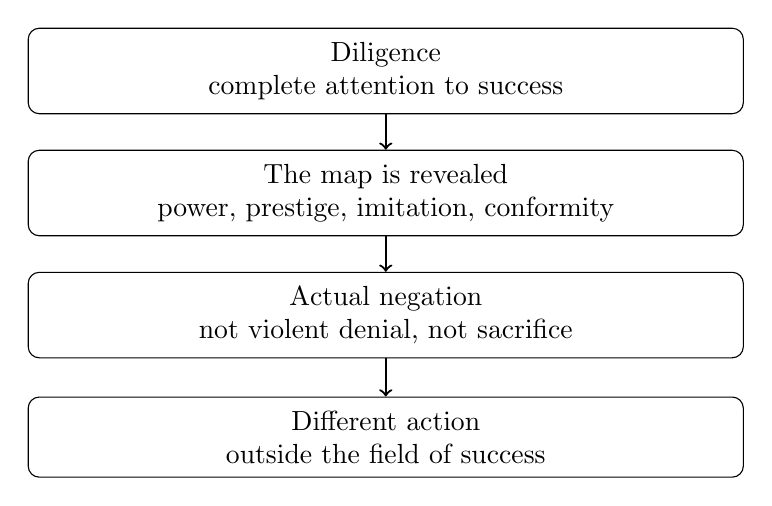
\begin{tikzpicture}[
  every node/.style={draw, rounded corners, align=center, text width=0.72\linewidth, inner sep=5pt},
  arrow/.style={->, thick}
]
\node (a) at (0,0) {Diligence\\complete attention to success};
\node (b) at (0,-1.55) {The map is revealed\\power, prestige, imitation, conformity};
\node (c) at (0,-3.10) {Actual negation\\not violent denial, not sacrifice};
\node (d) at (0,-4.65) {Different action\\outside the field of success};
\draw[arrow] (a) -- (b);
\draw[arrow] (b) -- (c);
\draw[arrow] (c) -- (d);
\end{tikzpicture}
\end{figure}

This also clarifies the ambiguity of ``self-denial.'' If self-denial means sacrifice, pain, or religious punishment, it distorts clear perception. If something is seen clearly, action is immediate. One does not need to maintain an act of denial. When danger is seen as danger, one does not keep deciding not to go near it.

Anderson's word ``practice'' briefly illuminates the same distinction. Practice, if it means repetition, cannot make this transformation. But if practice is heard in the older sense of praxis, direct act, then the act is not a temporal accumulation. The seeing and the doing are again one movement.

\section{Responsibility Without Delegation}

The final movement returns to freedom and responsibility in relationship. The dialogue now addresses a widespread evasion: we make others responsible. Politicians, priests, analysts, psychologists, professors, religious teachers, and traditions are given the burden, while the individual says, in effect, ``I only follow.''

Krishnamurti calls this irresponsibility:
\begin{equation}
\text{delegated responsibility}
\Longrightarrow
\text{irresponsibility}.
\end{equation}
Responsibility means total commitment to the challenge. A challenge is new; otherwise it is not a challenge. A crisis is new; otherwise it is not a crisis. Therefore the past cannot respond adequately to it.

The obstruction list is severe:
\begin{equation}
\text{fear}
\lor
\text{pleasure}
\lor
\text{routine}
\lor
\text{tradition}
\lor
\text{conditioning}
\Longrightarrow
\text{incomplete response}.
\end{equation}
The final condition follows:
\begin{equation}
\text{adequate response to challenge}
\Longrightarrow
\text{ending of the me as past}.
\end{equation}

Anderson's example from the \emph{Bhagavad Gita} sharpens the issue. Arjuna asks Krishna to tell him definitely what to do. In this reading, that request can itself be irresponsible: it asks another to carry the act of seeing. Responsibility is not obedience to an answer. It is total response to the challenge.

The lecture closes by distinguishing this from the ordinary phrase ``being responsible for my action.'' That phrase will need another inquiry, because it still may preserve the actor as a separate owner of action. Here responsibility has meant something more radical: responding wholly, without the past dictating the response.

\section{Summary}

We have followed the dialogue in its own order. Communication begins as a question about words, but quickly becomes a question about listening. Listening requires attention; attention opens the possibility of insight; insight is not delayed until the end. Communication becomes communion when two people meet the same problem with the same seriousness.

Seriousness is then separated from grim effort. It means total responsibility before an actual crisis. Responsibility is not the application of a plan, conclusion, belief, fear, pleasure, or tradition. It is adequate response to a challenge. That is why the observer cannot remain outside the observed: the world one tries to correct is not separate from the human being who has helped create it.

Finally, negation is shown to be neither suppression nor sacrifice. Actual negation is the seeing of the whole movement of success, power, immorality, or separation. In that seeing, the false thing ends; action is no longer in the old field. The lecture closes by refusing delegation. To respond completely, the self as past must end.